  \section[Logical Observation Identifier Names and Codes terminology\
  (LOINC\textsuperscript{\textregistered})] 
  {LOINC\textsuperscript{\textregistered}}
  \label{sec:loinc}
  
  \initial{L}\textit{ogical Observation Identifier Names and Codes terminology (LOINC )}\
 is a definitive standard for identifying clinical information in electronic reports.\
The LOINC database provides a set of universal names and ID codes\ 
for identifying laboratory and clinical test results in the context of existing\
 HL7, ASTM E1238, and CEN TC251 observation report messages. One of\
 the main goals of LOINC is to facilitate the exchange and pooling of results\
 for clinical care, outcomes management, and research. LOINC codes are\
 intended to identify the test result or clinical observation. Other fields in\
 the message can transmit the identity of the source laboratory and special\
details about the sample.\citep{_Vreeman_2013}\

 \begin{figure}[ht!]
    \centering
    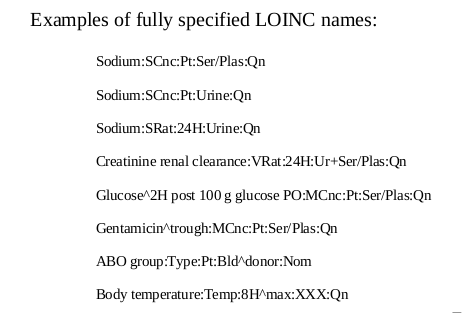
\includegraphics[scale=0.6]{loinc.png}
    \caption{Example of LOINC format\citep{_loinc_manual_2013}}
    \label{fig:loinc}
  \end{figure}  

\subsection{Global use}

Since then, many others have contributed translations. Currently,\
there are translation efforts underway in 18 countries to\
translate LOINC into 12 different languages, with translations into\
nine languages included in the most recent public LOINC release.\\

The freely available translations into many languages allows LOINC to\
be able to establish a global presence, and benefits the medical community by\
interoperable health information exchange around the world.\citep{vreeman_enabling_2012}\

 \subsection{Why would we use it for our application}

We should use it because of it's popular use currently around the world and the ability to adhere to community standards.\\

``LOINC has been widely adopted in both the public and private\
sectors, within the United States and more than 140 other countries.\
Several countries (including Brazil, Canada, Germany, the\
Netherlands, Mexico, and Rwanda) have adopted LOINC as a national standard,\
 and there are large health information exchanges using LOINC in Spain,\
 Singapore, and Korea as well. Within the US, LOINC has been adopted by\
 many health information exchanges, large national reference laboratories,\
 healthcare organizations, insurance companies, research programs, and national\
standards.''\citep{kroth_using_2012} 

 \subsection{How we can use it}

  There is a free software program developed by The Regenstrief Institute\
  called RELMA (the Regenstrief LOINC Mapping Assistant) which enables browsing\
  and searching the database, review accessory content for terms and map local\
  terms to LOINC \citep{kroth_using_2012} 

  \subsection{How is data stored}

LOINC is available as an Microsoft Access (.mdb) database file, a tab-delimited text file (.txt),\
 and also a comma delimited text file (.csv).\citep{_Vreeman_2013}\

 \subsection{Potential disadvantages}

 There are variations in the way LOINC is used for data exchange that result in some data not\
being truly interoperable across different enterprises. To improve its semantic interoperability, we need\
to detect and correct any contradictory knowledges. Also needed is detailed guidance on best practices\
for mapping from local codes to LOINC codes and for using LOINC\ 
codes in data exchange. \citep{lin_auditing_2012}



